\documentclass[a4paper]{article}

%use the english line for english reports
%usepackage[english]{babel}
\usepackage[portuguese]{babel}
\usepackage[utf8]{inputenc}
\usepackage{indentfirst}
\usepackage{graphicx}
\usepackage{verbatim}

\usepackage{listings}
\usepackage{float}
\usepackage{subfig}
\usepackage{hyperref}

\begin{document}
\setlength{\parindent}{3em}
\setlength{\parskip}{1em}
\setlength{\textwidth}{16cm}
\setlength{\textheight}{22cm}

\title{\Huge\textbf{Distrify}\linebreak\linebreak\linebreak
\Large\textbf{Relatório Final}\linebreak\linebreak
\linebreak\linebreak

\includegraphics[scale=0.1]{feup-logo.png}\linebreak\linebreak
\linebreak\linebreak
\Large{Mestrado Integrado em Engenharia Informática e Computação} \linebreak\linebreak
\Large{Programação em Lógica}\linebreak
}
\author{\textbf{Grupo Distrify\_4:}\\
João Guarda - 201303463 \\
Ricardo Lopes - 201303933 \\
\linebreak\linebreak \\
 \\ Faculdade de Engenharia da Universidade do Porto \\ Rua Roberto Frias, s\/n, 4200-465 Porto, Portugal \linebreak\linebreak\linebreak
\linebreak\linebreak\vspace{1cm}}

\maketitle
\thispagestyle{empty}

%************************************************************************************************
%************************************************************************************************

\newpage

\section*{Resumo}
Resumo sucinto do trabalho com 150 a 250 palavras (problema abordado, objetivo, como foi o problema resolvido/abordado, principais resultados e conclusões).

Foi proposto pelos docentes da unidade curricular Programação em Lógica o desenvolvimento em Prolog, linguagem geralmente utilizada para desenvolvimento de inteligência artificial e linguística computacional, de um jogo de tabuleiro para dois jogares.

Foram propostos alguns jogos dos quais escolhemos o Distrify. Sendo o jogo recente uma vez que foi publicado em 2015, estudamos o jogo desde o que era necessário para jogar, regras e forma como seria implementado em Prolog.

Foi implementado um motor de funcionamento do jogo tanto para um jogador como para dois sendo computadores ou não, utilizando a linguagem Prolog. A interface gráfica numa primeira fase foi desenvolvida utilizando apenas a consola no entanto numa segunda fase será desenvolvida numa outra unidade curricular (LAIG) uma interface em três dimensões utilizando o Prolog como meio de comunicação entre a parte lógica e a gráfica.

No final conseguimos atingir o objetivo: desenvolvimento da parte lógica de um jogo, de modo a ser possivel um futuro desenvolvimento ao nivel da interface gráfica. 

Concluimos que Prolog é uma linguagem muito interessante ao nível de implementação lógica neste caso de um jogo, pois permite estruturar de uma forma prática e eficaz o código em relação ao prévio planeamente lógico, isto é, antes de qualquer implementação prática.


\newpage

\tableofcontents

%************************************************************************************************
%************************************************************************************************

%*************************************************************************************************
%************************************************************************************************

\newpage

%%%%%%%%%%%%%%%%%%%%%%%%%%
\section{Introdução}

Este trabalho tem como objetivo desenvolver um jogo de tabuleiro para duas pessoas sendo que o desenvolvimento da parte lógica será através da utilização da linguagem Prolog e a implementação de uma interface gráfica adquada ao jogo, de modo a numa fase posterior possibilitar o desenvolvimento gráfico da aplicação baseando-se no Prolog como meio de comunicação entre diferentes ferramentas que permitem uma ligação entre a parte lógica e gráfica do jogo.

O relatório está estruturado de forma a dar a conhecer o jogo, primeiramente pela enumeração e explicação das suas regras, conceitos e objetivos depois o modo de implementação, a sua explicação lógica e estados de jogo e, por fim, é dada uma ideia da interface gráfica.

%%%%%%%%%%%%%%%%%%%%%%%%%%
\section{O Jogo Distrify}

Distrify é um jogo de tabuleiro, combinatorial e de conexão. Foi concebido a 22 de Agosto de 2015 por David Stoner.
É constituído por um tabuleiro quadrado de 9x9 a 19x19 quadrículas e por duas peças de cor diferente (branco e preto).
\subsection*{Regras}
O jogador com as peças de cor preta começa a jogar posicionando uma peça numa qualquer quadrícula do tabuleiro. Seguidamente, existem duas possibilidades:
\begin{enumerate}
\item Colocar uma peça numa qualquer quadrícula desde que não forme um \textit{\textbf{crosscut}}.
\item Colocar duas peças em quadrículas vazias, desde que não sejam adjacentes diagonalmente entre elas e não resultem num \textit{\textbf{triplet}} ou \textit{\textbf{crosscut}}.
\end{enumerate}
De realçar que \textbf{haverá sempre uma jogada válida}, pelo que os jogadores \textbf{não podem passar a vez}.

\subsection*{Conceitos}
\begin{itemize}
\item \textit{\textbf{crosscut}}: quando se verifica uma cruz constituída pelo mesmo número de peças de ambos os jogadores. Vi-de fig.1.
\item \textit{\textbf{triplet}}: quando 3 peças estão seguidas na horizontal, na vertical ou diagonalmente.
\item Duas peças da mesma cor são consideradas \textbf{ligadas} quando estão adjacentes horizontalmente, verticalmente ou diagonalmente.
\end{itemize}
\begin{figure}[H]
	\centering
	
\includegraphics[scale = 0.3]{images/crosscut.png}
	\caption{Padrão de \textit{crosscut}}
	\label{fig:crosscut}
\end{figure}
\subsection*{Objetivo}

O jogador com peças pretas ganha se, a qualquer momento, se verificar um caminho contínuo de peças ligadas entre elas desde o topo do tabuleiro até à base (Fig.2 (a)).
\par
O jogador com peças brancas ganha se a qualquer momento se verificar um caminho contínuo de peças ligadas entre elas desde o lado esquerdo até ao lado direito do tabuleiro (Fig.2 (b)).

\begin{figure}[H]
	\centering
	\subfloat[Caminho (a vermelho) de vitória das peças pretas.]{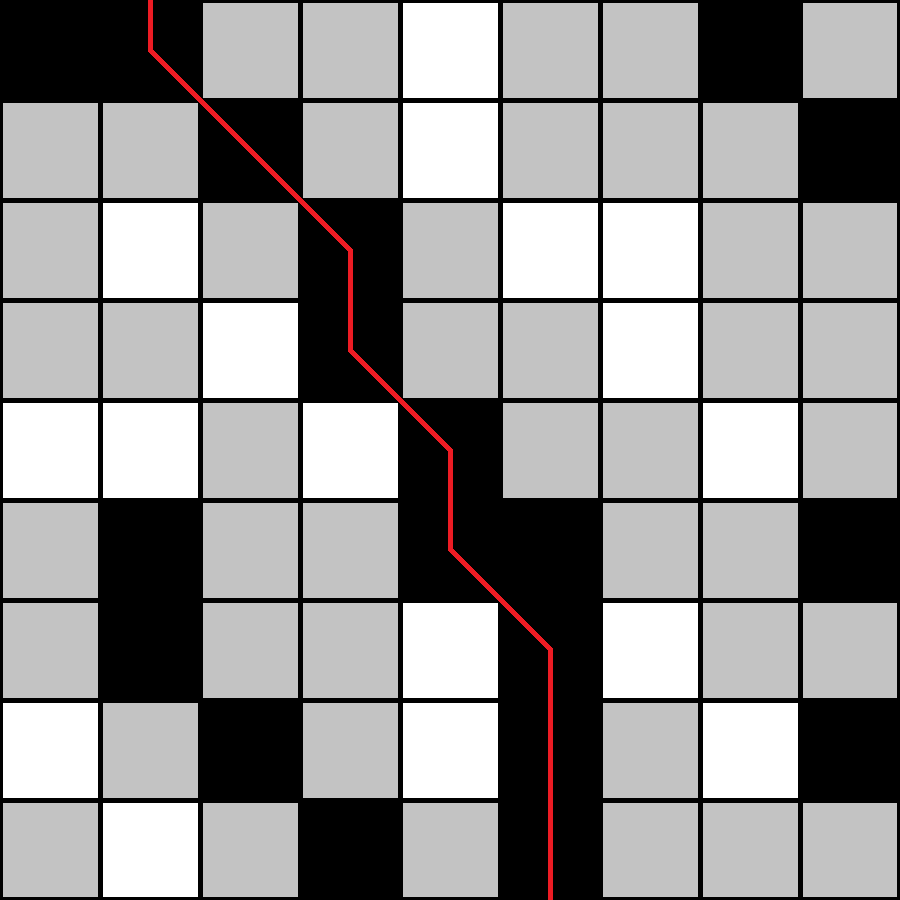
\includegraphics[width=0.3\textwidth]{images/blackWin.png}\label{fig:f1}}
	\hfill
	\subfloat[Caminho (a vermelho) de vitória das peças brancas.]{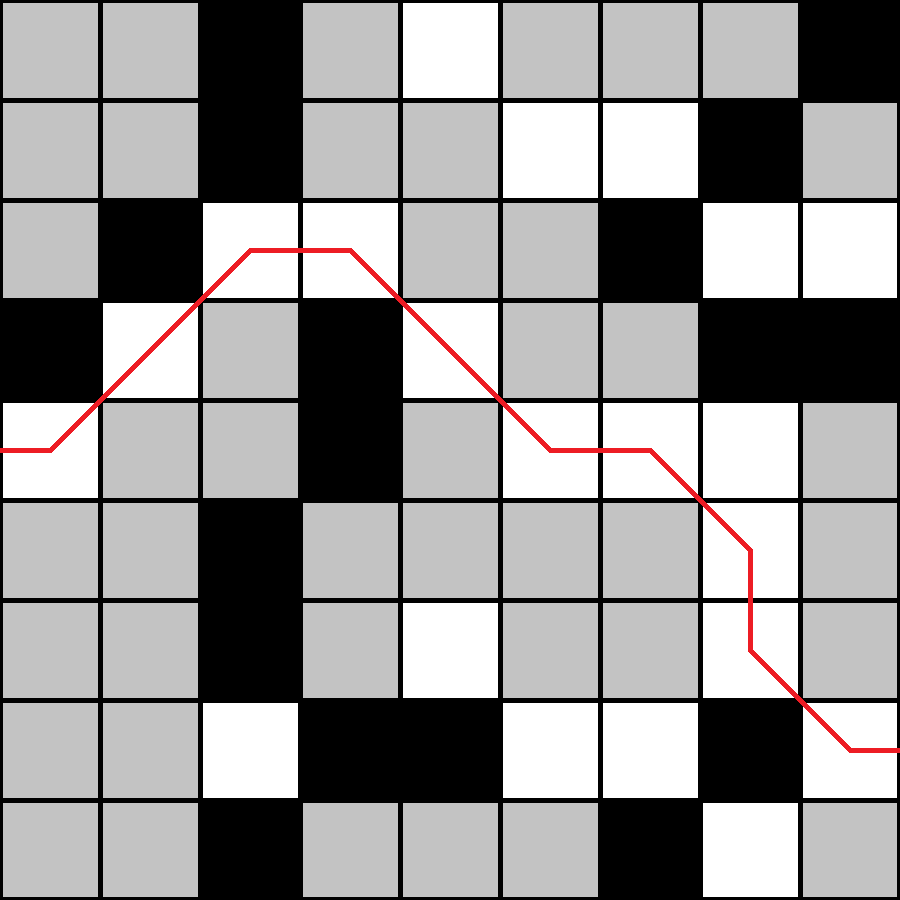
\includegraphics[width=0.3\textwidth]{images/whiteWin.png}\label{fig:f2}}
	\caption{Exemplos de vitórias.}
\end{figure}

%%%%%%%%%%%%%%%%%%%%%%%%%%
\section{Lógica do Jogo}

Descrever o projeto e implementação da lógica do jogo em Prolog, incluindo a forma de representação do estado do tabuleiro e sua visualização, execução de movimentos, verificação do cumprimento das regras do jogo, determinação do final do jogo e cálculo das jogadas a realizar pelo computador utilizando diversos níveis de jogo. Sugere-se a estruturação desta secção da seguinte forma:

\subsection{Representação do Estado do Jogo} Pode ser idêntico ao descrito no relatório intercalar.)

\subsection{Visualização do Tabuleiro} (Pode ser idêntico ao descrito no relatório intercalar.)

\subsection{Lista de Jogadas Válidas} Obtenção de uma lista de jogadas possíveis. Exemplo: \textit{valid\_moves(+Board, -ListOfMoves)}.

\subsection{Execução de Jogadas} Validação e execução de uma jogada num tabuleiro, obtendo o novo estado do jogo. Exemplo: \textit{move(+Move, +Board, -NewBoard)}.

\subsection{Avaliação do Tabuleiro} Avaliação do estado do jogo, que permitirá comparar a aplicação das diversas jogadas disponíveis. Exemplo: \textit{value(+Board, +Player, -Value)}.

\subsection{Final do Jogo} Verificação do fim do jogo, com identificação do vencedor. Exemplo: \textit{game\_over(+Board, -Winner)}.

\subsection{Jogada do Computador} Escolha da jogada a efetuar pelo computador, dependendo do nível de dificuldade. Por exemplo: \textit{choose\_move(+Level, +Board, -Move)}.


%%%%%%%%%%%%%%%%%%%%%%%%%%
\section{Interface com o Utilizador}

Descrever o módulo de interface com o utilizador em modo de texto.


%%%%%%%%%%%%%%%%%%%%%%%%%%
\section{Conclusões}
Que conclui deste projecto? Como poderia melhorar o trabalho desenvolvido?

Concluimos que a linguagem Prolog é muito útil e propicia no desenvolvimento lógico de um jogo, permitindo estruturar de uma forma mais conseguida a ideia do jogo em si.

\clearpage
\addcontentsline{toc}{section}{Bibliografia}
\renewcommand\refname{Bibliografia}
\bibliographystyle{plain}
\bibliography{myrefs}

\newpage
\appendix
\section{Nome do Anexo}
Código Prolog implementado devidamente comentado e outros elementos úteis que não sejam essenciais ao relatório.

\end{document}
